% https://tex.stackexchange.com/a/762107/322482
\documentclass[tikz,border=1cm]{standalone}
\usetikzlibrary{arrows.meta,backgrounds}
\usepackage{fourier}
\begin{document}
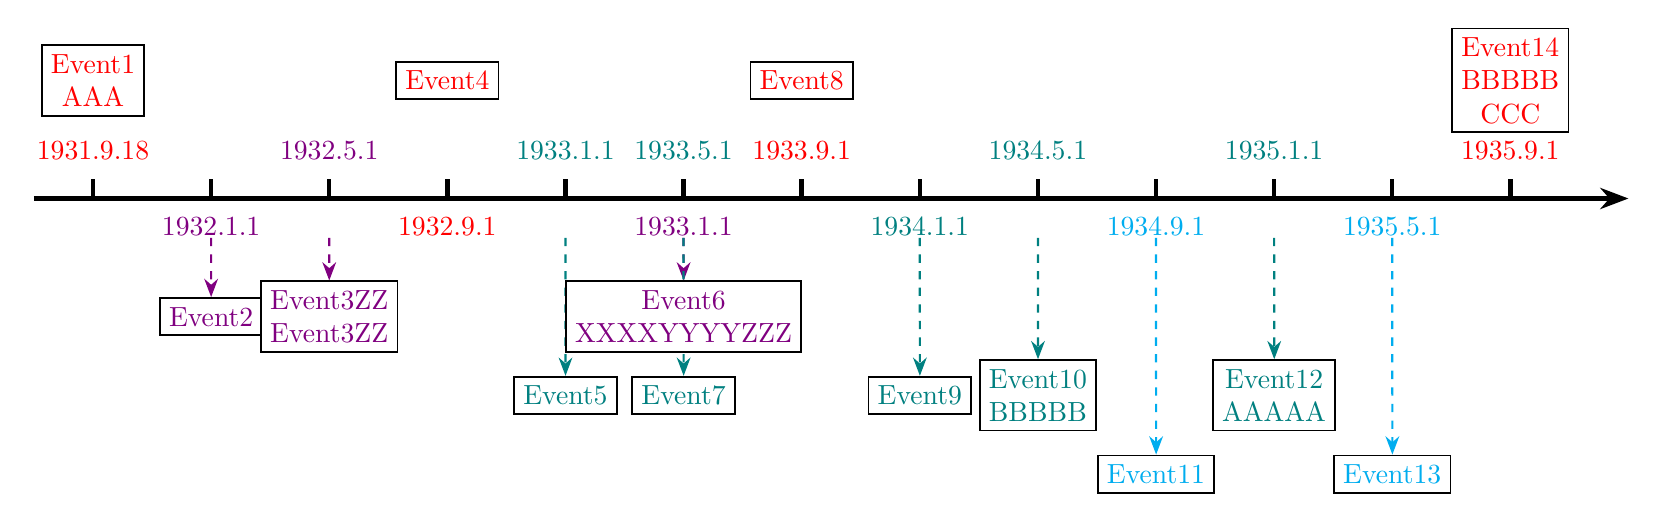
\begin{tikzpicture}[xscale=1.5,>=Stealth]
  \draw[ultra thick,->] (-.5,0) -- (13,0);
    \def\above{above}
    \foreach \xpos/\timeline/\timepos/\mycolor/\contentyshift/\eventcontent[count=\nn] in {%
        0/{1931.9.18}/above/red/1.5cm/{Event1\\AAA},
        1/{1932.1.1}/below/violet/-1.5cm/{Event2},
        2/{1932.5.1}/above/violet/-1.5cm/{Event3ZZ\\Event3ZZ},
        3/{1932.9.1}/below/red/1.5cm/{Event4},
        4/{1933.1.1}/above/teal/-2.5cm/{Event5},
        5/{1933.1.1}/below/violet/-1.5cm/{Event6\\XXXXYYYYZZZ},
        5/{1933.5.1}/above/teal/-2.5cm/{Event7},
        7/{1934.1.1}/below/teal/-2.5cm/{Event9},
        6/{1933.9.1}/above/red/1.5cm/{Event8},
        8/{1934.5.1}/above/teal/-2.5cm/{Event10\\BBBBB},
        9/{1934.9.1}/below/cyan/-3.5cm/{Event11},
        10/{1935.1.1}/above/teal/-2.5cm/{Event12\\AAAAA},
        11/{1935.5.1}/below/cyan/-3.5cm/{Event13},
        12/{1935.9.1}/above/red/1.5cm/{Event14\\BBBBB\\CCC}%
    }{%
        \ifx\timepos\above
            \draw[ultra thick] (\xpos,0) --+(0,.25) 
            node[\timepos=.1cm,text=\mycolor,align=center] {\timeline};
        \else
            \draw[ultra thick] (\xpos,0) node[\timepos=.1cm,text=\mycolor,align=center] {\timeline} --++(0,.25);
        \fi 
        \node[draw,semithick,fill=white,yshift=\contentyshift,align=center,text=\mycolor,anchor=center] at (\xpos,0) (content-\nn){\eventcontent};
        \begin{scope}[on background layer] 
            \ifdim\contentyshift<0pt\relax
                \draw[thick,dashed,->,\mycolor] (\xpos,-0.5) -- (content-\nn.north);
            \fi
        \end{scope}
    }
\end{tikzpicture}
\end{document}